\chapter{Displacement}
\label{Chapter:Displacement}
\begin{flushright} 
\textit{"The eye altering, alters all."\\ -William Blake, The Mental Traveller}
\end{flushright} 
\begingroup
    %\vspace*{\beforechapskip}% 
    %\smash{\rule{2.6pt}{25mm}}
\textit{Dislocated sensors, changing their position during use, are very problematic for realistic activity recognition.
This chapter motivates why dealing with sensor displacement within a body part is crucial. We discuss the theoretical background, point out alternative approaches, and present a set of heuristics that significantly increase the robustness of motion sensor-based activity recognition with respect to sensor displacement. We show how, within certain limits and with modest quality degradation, motion sensor-based activity recognition can be implemented in a displacement tolerant way. We describe the physical principles that lead to our heuristic and evaluate them on a set of synthetic lower arm motions. These motions are well suited to illustrate the strengths and limits of our approach. We extend the evaluation on a realistic modes of locomotion problem (sensors on the upper leg) and finally on a set of exercises performed on various gym machines (sensors placed on the lower arm). Our heuristic raises the displaced recognition rate from 24\% for a displaced accelerometer (96\% accuracy when not displaced) to 82\%.
}
\\\\
Kunze, K. and Lukowicz, P. Dealing with sensor displacement in motion-based on-body activity 
recognition systems. \textit{In Proceedings of the 10th Conference on Ubiquitous computing.} Seoul, Korea, September, 2008. (Acceptance rate: 18\%). 
\vskip\onelineskip
\begin{adjustwidth}{}{-\chapindent}%
\hrulefill   
\end{adjustwidth}\endgroup
\vskip\onelineskip
Even if we know the coarse grain on-body placement of a device, it's often not possible to perform activity recognition. On-body motion sensors can just provide crude contextual information in realistic scenarios without considering orientation changes and displacement~\cite{Lester:2006p856,Maurer:2006p1533}. 

We define displacement as dislocation within a body part, excluding orientation issues. Take the example of an mp3 player attached to the upper arm. If it shifts in position up or downwards, the methods and heuristics in this chapter apply. If however the device rotates around the arm and shifts, the heuristics in this chapter need to be accompanied by some methods to deal with orientation change described later.

Today, most device attachment methods leave a lot of room for placement within a body part. Thus, a user can place arm holders for mp3 players, often used for jogging, almost anywhere on the upper or lower arm. 
Integration of sensors in clothing can ensure that sensors end up on a certain body part. However, one cannot ensure a specific placement on that body part. Even a tight fitting sleeve can be rolled up or twisted, completely changing the placement of any integrated sensor.

Unfortunately, the within body part placement issue cannot be solved with simple calibration gestures for motion sensors. As explained in section~\ref{sec:pyhsical}, the gravity component of an accelerometer does not depend on the position within a body part. Thus, a static calibration gesture is not sufficient. Instead, motions must be performed with {\em different, exactly defined speeds and trajectories}. In general, we cannot expect the user to perform such exactly defined motions with sufficient reliability. 

\section{Sensor Displacement Impacts}
\label{dis:impacts}
Displacement within a body part is crucial for motion-sensor-based
activity recognition. Yet, displacement effects other sensing modalities to a much lesser degree. For those, on-body placement and orientation changes are more critical (see Sections 3.2 and 5.2). Therefore, non-motion-based modalities are not discussed in this chapter.

Motion sensors, in particular accelerometers, are a common type of
body worn sensors for activity recognition. Following the original
work by Randell, Van Laerhofen and
Mantyjarvi~\cite{randell2000caa,vanlaerhoven2000swt,mantyjarvi2001rhm},
there have been numerous publications dealing with applications
ranging from dancing sign language recognition, tracking of every day
activities to industrial maintenance and mental health related
applications
~\cite{aylward2006swc,brashear2003ums,vanLaerhoven:2007p1441,
Krause:2006p1527,prevasiveskoda,westeyn2005rma}.


\begin{figure*}[t]
\centering   
\includegraphics[scale=0.30]{sleeves.pdf}
\caption[Displacement accelerometer signal example]{Signal example for displacement within a body part. You see one axis of
two acceleration signals from the same device mounted on the upper arm, the
only difference being that the device is displaced by 10 cm.}
\label{fig:Dexample}
\end{figure*}

The vast majority of research in this area 
assumes well defined, fixed sensor locations. This is particularly
important for activity recognition related to arm and hand motions.
As depicted in Figure~\ref{fig:Dexample}, displacement within a
body part highly affects the characteristics of an accelerometer signal.
%Gyroscopes are a bit more robust to displacement changes, we will present
%details later. 

Being able to drop the requirement for a 'well defined fixed position' and
building systems that can deal with sensor displacement has two major
advantages:

\begin{itemize}
\item Robustness. During long-term deployment, sensor
  shifts will eventually happen.  Enabling the system to continue
  working correctly despite sensor shifts is a significant
  improvement to robustness.
\item Better usability and user acceptance. Today, many mobile
  appliance are already equipped with sensors. Sensor encapsulation into
  clothing or unobtrusive attachment e.g., as "buttons"
   has been demonstrated~\cite{roggen2006smn}. It is thus often taken
  for granted that users  can be easily equipped with sensors in every day
  situations.  This does not imply, however, that the user can be 
 expected to reliably and firmly fix the sensors to narrowly defined on-body locations.
\end{itemize}

In summary, regarding the three sub-categories described in the introduction ('on-body part' placement, displacement and sensor orientation changes), displacement is the most difficult to handle. It is so far an unsolved problem. This chapter addresses possible solutions. 


\section{Related Work}

To our knowledge there is no other work directly targeting the problem of 'within body part' displacement for motion sensors. The standard practice to deal with displacement is to take robust, aggregate features, which can either only be used for very simple recognition tasks or lead to a significant degradation in recognition performance~\cite{Lester:2006p856,Krause:2003p1536,Borriello:2006p1201}. Yet, there is some complimentary work, trying to tackle the problem more directly.

Van Laerhoven presented a study to explore the trade-offs between 
single on-body sensors with predefined, well-known placement 
and an increasing quantity of sensors with decreasing information quality 
(placement accuracy)\cite{vanLaerhoven:2008p1442}.  
Zinnen showed an innovative way to use rest periods in accelerometer signals 
for detection of non-repetitive tasks,
which is based on some of the principles presented below in section~\ref{sec:pyhsical}~\cite{Zinnen:2008p631}. 
Lester uses acceleration signatures to 
determine that a set of devices is being
carried by the same person~\cite{Lester:2004p738}. 
There is also some work on evaluating
the suitability of different on body locations
for activity recognition~\cite{Maurer:2006p1533}. A platform with 
multiple sensors (in addition to mere motion sensors) has been investigated 
with respect to on-body location invariance of activity
recognition~\cite{Lester:2006p856}.
Forster et. al. utilize dedicated hardware with multiple accelerometers to track displacement changes online~\cite{Forster1,Forster2}.


\section{Idea and Contributions}
Although we did not discover an exact solution, 
we present a set of heuristics that significantly increase the robustness of motion
  sensor-based activity recognition with respect to sensor
  displacement within a single body part. We show how, within
  certain limits and with modest quality degradation, our heuristics  
  allow motion sensor based activity recognition to be implemented 
  in a displacement tolerant way. Thus,
  within a single body part, we demonstrate reliable recognition at
  locations different from those on which the sensor was trained. 
Our approach is based on three observations:
\begin{enumerate}
\item The signal of a body-worn accelerometer is the sum of three
  components: acceleration due to rotation,
  acceleration due to translation and acceleration due to orientation
  with respect to gravity. Of those three only the first one,
  acceleration due to rotation, is sensitive to sensor displacement
  within a single body part. We explain the underlying physical considerations 
in detail in Section~\ref{sec:pyhsical}.
\item The accelerometer signal segments dominated by rotation can be identified. 
  These segments are possibly 'contaminated' with displacement related noise.
\item Gyroscopes are more insensitive to displacement within a
  single body part. However, they provide only information on
  rotation, ignoring translations and vertical orientation.   
\end{enumerate}

From the above observations, it follows that combining a gyroscope with an
accelerometer removes some placement sensitivity, as the accelerometer can 
ignore all signal frames dominated by rotation , while retaining 
 most of the relevant information. In fact, sometimes just an accelerometer
ignoring the 'rotation-contaminated' frames is enough for
more displacement tolerant recognition. 
Additional measures we propose are the use of heavily low pass 
filtered acceleration signals and training the system on 
two sensors corresponding to the 'worst
possible displacement'.

The main validity limits of our heuristics are (1) a rigid
body approximation of human body parts and (2)
the assumption that the  bulk of the discriminative information is 
not in signal segments that contain simultaneously
performed fast rotations, significant translations or changes in
vertical orientation. 

In the rest of the chapter, we describe how our heuristics can
be  derived from  basic physical considerations. Next we apply these heuristics
to a set of "synthetic" gestures that are well suited to demonstrate
the strengths and limits of our approach. 
Finally, we present an evaluation on two real life
recognition tasks. The first task is an extended modes of locomotion
problem using upper leg mounted sensors. The second is a set of gym
exercises classified using sensors mounted on the lower arm.
On this set our heuristics improve recognition rates for displaced
sensors from 24\% using a displaced accelerometer( 96\% recognition
when not displaced) to 82\%. On other examples the displaced
recognition rates raise from around 60\% to over 90\%.

\section{Physical Considerations}
\label{sec:pyhsical}

To better understand our approach, 
we discuss the physics background, introducing 
a rigid body approximation and deducing consequences from this
assumption regarding motion sensors.

\subsection{The Rigid Body Approximation}
\label{sec:rigid}

\begin{figure}[t]
    \begin{center}
    \subfloat[]{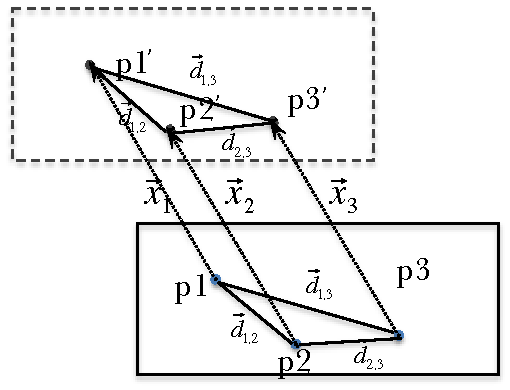
\includegraphics[height=1.8in]{translation1.pdf}
    	\label{fig:translation}}
    \subfloat[]{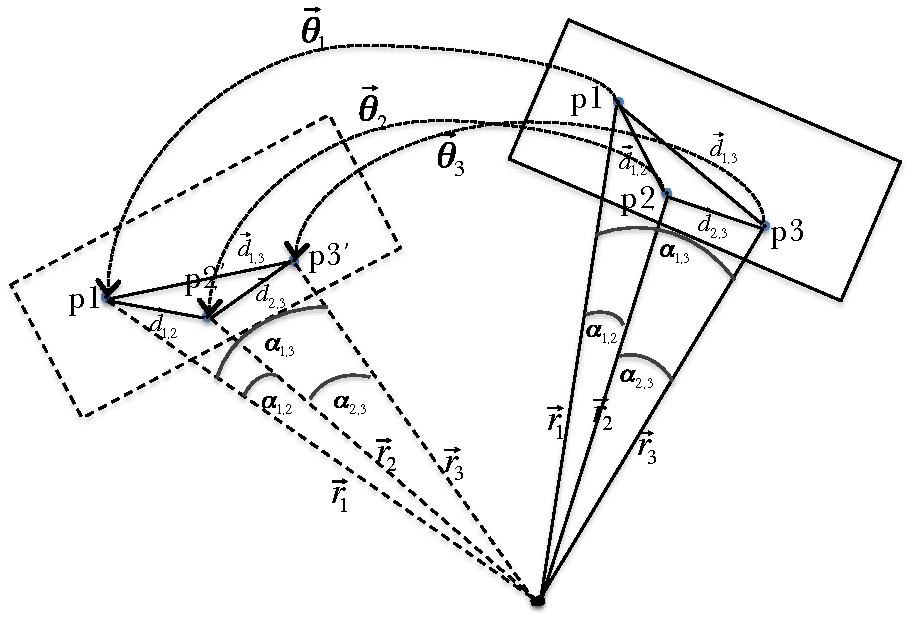
\includegraphics[height=2.1in]{rotation1.pdf}
    	\label{fig:rotation}}
      \end{center}
\caption[Rigid body translation and rotation]{Rigid body translation~\ref{fig:translation} and rotation~\ref{fig:rotation}}
\label{fig:physics}
\vspace{-10pt}
\end{figure}

A common approximation used in modeling human body motion is
that of rigid segments connected by joints which allow rotation
around  one (e.g. elbow) or more axes (e.g. wrist). 
In simple terms, such an approximation is equivalent to a 'stick figure' 
representation used in many animations. In exact terms, a rigid body is 
an ideal solid body of finite size for which the relative position of any 
two given points remains constant in time regardless of external forces exerted
on it. Any motion of a rigid body can be described as a combination
of a translation and a rotation.

\begin{figure*}[t]
\centering   
\includegraphics[scale=0.4]{translation-example.pdf}
\caption[Rigid body translation example]{Signal sample from a rigid body translation. The gyro signal
is on the top right and shows little to no activation. The accelerometer
signal is below and is fairly the same for both sensors.}
\label{fig:trans-example}
\end{figure*}

\begin{figure*}[t]
\centering   
\includegraphics[scale=0.4]{rotation-example.pdf}
\caption[Rigid body rotation example]{Signal sample from a rigid body rotation. As seen, the gyros, on the
top right show some activation and are more or less identical.
The accelerometer reading for the two sensors differ.}
\label{fig:rot-example}
\end{figure*}

Although human joints posess only rotational degrees of freedom, 
a motion combining simultaneous rotation at two different joints can 
have the effect of a translation (e.g. shifting your lower arm through 
a combined elbow and shoulder motion). Additionally, motions involving more than
one joint can lead to rotations around axes that are not identical
to any of the involved joints. Regarding arm motions, such axes are 
often close to the torso.

\paragraph{Rigid Body Translation}
During a translation every point in a 
rigid body is moved by exactly the same {\em vector} with exactly the
same speed and acceleration. 
This is illustrated in figure \ref{fig:translation}. The figure shows a rigid body
with three arbitrary points $p_1,p_2,p_3$. The relative
positions of those points are given by the difference vectors
$\vec{d}_{1,2},\vec{d}_{1,3},\vec{d}_{2,3}$. We assume that the body is
translated (=moved in a straight line) randomly which
results in  $p_1,p_2,p_3$  being moved by a corresponding
vectors $\vec{x_1}, \vec{x_2},\vec{x_3}$.  Per definition of a rigid body 
the relative positions given 
by $\vec{d}_{1,2},\vec{d}_{1,3},\vec{d}_{2,3}$ must
remain unchanged. This is only possible if all the points are moved
by exactly the same vector:
\begin{equation}
\vec{x_1}=\vec{x_2}=\vec{x_3}
\end{equation}
 This is valid
independently of the translation distance and the time it
took. Thus, given a translatory motion, at any point in time during
this motion, all points of a rigid body will have moved by
exactly the same vector. A signal example is given in figure~\ref{fig:trans-example}
to visualize this fact.

This is also valid for infinitesimally small
time intervals which implies that at any given point in time the speed
and with it the acceleration vectors will also be the same for all points.
The velocity and acceleration equation are given bellow.

\begin{equation}
v(t) = {\lim_{\Delta t \to 0}{{x(t+\Delta t)-x(t)} \over \Delta t}={{d}x \over dt}}
\end{equation}


\begin{alignat}{3}
a = \frac{d v}{dt} 
 \end{alignat}


\paragraph{Rigid Body Rotation} In an analogous way it can be shown that 
{\em  angular velocity  vector} (and  angular acceleration)
are the same for all points of a rigid body during a rotation around an
arbitrary point in space. To illustrate this, figure~\ref{fig:rotation} 
shows a rigid body in which three arbitrary
points $p_1,p_2,p_3$ and an arbitrary
center of rotation $r$ are marked. The vectors connecting each point to 
the center of rotation are labeled as $\vec{r_1}, \vec{r_2},\vec{r_3}$, 
their relative angles as $\alpha_{1,2},\alpha_{1,3},\alpha_{2,3}$. 
We consider a rotation around $r$ which results in 
 $p_1,p_2,p_3$ being rotated by $\theta_1,\theta_2,\theta_3$. 
Since per definition of a rigid body
after the rotation the relative positions of the three points  given
by $\vec{d}_{1,2},\vec{d}_{1,3},\vec{d}_{2,3}$ must be unchanged, the
relative angles between vectors connecting them to the center of
rotation $\alpha_{1,2},\alpha_{1,3},\alpha_{2,3}$  must also be
unchanged. This is only possible if all three points are
rotated by the same angle: 
\begin{equation}
\theta_1=\theta_2=\theta_3
\end{equation}
As for translation considering infinitesimal time
periods, the angular speed $\omega$ and acceleration must
also be the same for all three points. 

In summary, during a rotation of a
rigid body around an arbitrary point in space a gyroscope will 
produce the same signal no matter where in the rigid body it is placed.
As will be explained later, this does not apply to accelerometers
since  different points in a rigid body in general
experience a  {\em different, non zero acceleration vector} during a rotation.
Again we show a small signal example for illustration in Figure~\ref{fig:rot-example}.

%Clearly a rotation and a translation can be overlaid in a single
%motion and executed simultaneously. In this case, the velocities and
%accelerations in each point are the sum of the values that are caused
%by the translation and the rotation. 

\paragraph{Limits of the Rigid Body Approximation}
Obviously, the individual segments of the human body are not
rigid bodies. Deformation of soft tissue, skin motion and
muscle activity associated with most motions all lead to
deviations. However, as will be underscored by subsequent experiments
(see Section \ref{sec:experiments}), for many sensor positions and motions
it is a valid approximation. The main deviations from the rigid body
approximation can be observed in the following situations.

\begin{enumerate}
\item During short, intensive acceleration and  follow up vibrations
  soft 'wobbly' parts (fat, soft muscles) are deformed in a non rigid
  way. To deal with such deviations the system can simply discard such vibrations or
  apply the previously mentioned low-pass filtering.
\item  When active muscles change shape. In particular large muscles
  will cause motion signals incompatible with the rigid body
  approximation. Thus, one should avoid placing sensors
  directly on top of a well developed biceps. Fortunately, such
  placement is often not very convenient and users will most probably avoid it.
\item The lower arm rotation parallel to the axis of the arm will
  affect sensors fixed to the wrist in a significantly different way
  than sensors near the elbow. The wrist sensor rotates perfectly with the
  wrist, whereas the elbow sensor will do so to a much lesser
  degree. Gestures, relying on such rotations as an important
  discriminative information present a problem for our location invariant recognition,
  as illustrated by our 'synthetic gestures' evaluation in Section~\ref{sec:experiments}. 
\end{enumerate}

\subsection{Acceleration during Rigid Body Rotation}
During a pure translation, gyroscopes will provide no signal at all
(there is per definition no rotational component) while accelerometers will all give the same readings no matter where they are placed (see figure~\ref{fig:trans-example} for an example). 

As already pointed out, in a rigid body
all points are rotated with the same angular velocity ($\omega$) and experience the same angular
acceleration $\alpha$.   Thus, the gyroscope signal is invariant with
respect to sensor displacement. 

To understand the effect of sensor displacement during rotation on the
accelerometer signal we
need to revisit some basic physics.
During a rotation with the  angular velocity $\omega$, 
the linear velocity $v$ of each point of the rigid
body depends on the distance to the center of
rotation $r$. The further the point is located from the center, the larger the
circle it needs to travel and, consequently, the faster it moves. The speed is defined as: 
\begin{equation}
\label{eq:speed}
v=\omega r
\end{equation}
The important thing to remember when looking at the above equation is
that $v$ designates the speed traveled along a circle. This means
that, although the scalar value of the speed is constant (if $\omega$
remains constant), to follow the circle each point of a rotating
rigid body constantly has to change its direction\footnote{The
  vector $\vec{v}$ is parallel to the tangent of the circle in each point
of the rotation}.  Such a change of
direction requires acceleration. The direction of the acceleration
is parallel to the radius of the circle. The magnitude of this
acceleration depends on the
speed (the faster a point travels the more force is required to change
direction) and with it on the distance for the center.  The magnitude
of 
linear acceleration $a_{\omega}$ due to constant angular velocity  $\omega$  in a point at the distance $r$ from the center of
rotation is given by: 
\begin{equation}
\label{eq:centrifugalx}
a_{\omega}=\omega^2r
\end{equation}
This gives
us the first source of acceleration  during a rotation of a
rigid body. It is often referred to as centripetal acceleration.
The second potential source stems from changes in the
rotation speed. Since the linear speed is proportional to the angular
velocity and the distance to the center (equation \ref{eq:speed}),
it follows that the linear acceleration $a_{\alpha}$ associated with a change of
angular velocity is proportional to the angular acceleration
($\alpha$) and the distance from the center $r$: 
\begin{equation}
\label{eq:tangential}
a_{\alpha}=\alpha r
\end{equation} 
This component is called tangential acceleration. 

Since the centripetal acceleration and the tangential
acceleration are perpendicular, not parallel, the scalar 
values given above cannot simply be added to get 
the total magnitude of acceleration (the Euclidian norm of
the acceleration vector).  For the sake of simplicity we will just
deal with each of them separately \footnote{Since the two are
  perpendicular their contribution to the norm of the acceleration
  $a_{combined}$ is given by $\sqrt{\omega^4r^2+\alpha^2 r^2}$}
Another simplification is to ignore the Coriolis 
force which acts on objects  moving along the rotation axis. 
By moving more than one joint at a time, it is certainly possible to construct 
motions of human body parts for which the coriolis acceleration plays a 
significant role. Yet, motions where this is a relevant component are
rare and will not be discussed it in this chapter.

\subsection{Consequences for Displaced Sensors}
What does the above mean for the noise introduced by displacing a
sensor within a single, rigid body segment?
As already stated a gyroscope signal is displacement-invariant, thus, there is no
need to considered it further. 
For an acceleration signal we need to differentiate between three
contributions: (1) the contribution caused by orientation with respect
to gravity, (2) the contribution caused by translations and  (3)
contribution caused by rotation. As explained above, the first two are
location invariant. Only the rotation component is location-sensitive. 

\paragraph{Displacement Noise in Rotation Related Acceleration}
Given two points of a rigid body: one with a distance $r_1$
from the center of rotation and the second one with a distance of
$r_2$, we can compute the  acceleration components
resulting from constant rotation $a_{\omega,1},a_{\omega,2}$ and from
angular acceleration $a_{\alpha,1},a_{\alpha,2}$ using equations
\ref{eq:centrifugalx} and \ref{eq:tangential}. 
Thus, the signal difference attributed to sensor displacement can be
computed as
\begin{eqnarray}
\label{eq:diff_centrifugal}
a_{\omega,1}-a_{\omega,2}=\omega^2r_1-\omega^2 r_2=\omega^2(r_1-r_2)
\\
\label{eq:diff_tangential}
a_{\alpha,1}-a_{\alpha,2}=\alpha r_1-\alpha  r_2=\alpha(r_1-r_2)
\end{eqnarray} 
How relevant this difference is to the recognition not only depends on its
absolute  magnitude, but also on the signal to noise ratio. This is
the ratio of the original signal ($a_{\omega,1}$ or
$a_{\alpha,1}$) to the difference caused by displacement
($a_{\omega,1}-a_{\omega,2}$ or $a_{\alpha,1}-a_{\alpha,2}$).  It can
be computed from equations \ref{eq:diff_centrifugal} and
\ref{eq:diff_tangential}:
\begin{eqnarray}
\label{eq:diff_centrifugal1}
\frac{a_{\omega,1}-a_{\omega,2}}{a_{\omega,1}}=\frac{\omega^2(r_1-r_2)}{\omega^2
  r_1}=\frac{r_1-r_2}{r_1}
\\
\label{eq:diff_tangential1}
\frac{a_{\alpha,1}-a_{\alpha,2}}{a_{\alpha,1}}=\frac{\alpha(r_1-r_2)}{\alpha
  r_1}=\frac{r_1-r_2}{r_1}
\end{eqnarray}
The above is a very compelling result. It shows that sensor
displacement noise during rotational movement depends only on the amount of
displacement {\em with respect to the center of rotation}. It is
independent of the actual angular velocity or angular acceleration.  

\paragraph{Consequences for the Recognition} The previous paragraph dealt with the distortion of the acceleration signal
related to rotation, as the other components are not affected by
displacement. A naive idea for the design of an displacement
invariant recognition system is to try to ignore the rotation
related component of the acceleration signal and use only the 
translation and vertical orientation related components.

Unfortunately, in general\footnote{The general case assumes that there
  is no additional information such as 
further sensors in different locations on the same body part or appropriate high level knowledge about the
form and constraints of the motion}, it is theoretically not possible  
to decompose an acceleration signal into the three components above. 
Note that this remains true
even if we combine an acceleration sensor with a gyroscope.  The
gyroscope will indicate the presence and speed of rotation.
As shown in equation~\ref{eq:diff_centrifugal}, to compute the
acceleration we need the distance from the center of rotation, which we, however,
do not know.

Fortunately, although we do not know the exact radius of the
rotation, we know that it is bounded by the dimensions of the human
body. While rotational motions with very high radius can be
constructed, for most human limb motions the center of rotation is
somewhere close to the torso.  This means, that for a given rotation
speed, the acceleration is unlikely to exceed a certain value. Therefore, 
we can use the ratio of rotation velocity measured by
a gyroscope to the norm of the acceleration vector computed from the
acceleration sensor signal, to determine if the acceleration signal is
rotation dominated or not. A high acceleration with a relatively low
measured angular velocity is a good indication of the signal not being
dominated by rotation. On the other hand, high angular velocity with
low or moderate acceleration is an indication of a rotation dominated
motion.

The ratios of angular velocity to acceleration norm
signifying the transition between rotation and translation dominated signal
depend on the typical rotation radius and with it on the 
motions relevant to the specific recognition task. They have to be learned 
during training. We will show an example in the next paragraph. 

 Thus, while we can not separate the individual
 components of a given acceleration signal, it is possible to estimate
 with reasonable probability which signal frames are dominated by
 rotation and which are not. We can then discard the rotation
 dominated frames, which are sensitive to displacement and use
 only the ones dominated by translation and/or
 vertical orientation.  In a sensor setup with a gyroscope we can
 try to substitute the rotation for the discarded acceleration
 frames to retain rotation related information. 

Another interesting consideration relates to the vertical orientation
component of the acceleration signal. Any (non free falling) object on Earth is
subject to a constant 9.81 $m/s^2$ acceleration. This means that if the norm
of the acceleration signal is close to 9.81, then the signal is likely
to be dominated by the vertical orientation component. Clearly, this heuristic 
is not always valid. We can imagine a
situation when an object is free falling while experiencing a 9.81 $m/s^2$
side acceleration. However this is a rare occurrence, and the above
assertion is mostly valid (as will be
underscored by the experiments in the next section).   

\subsection{In Summary}
To conclude the theoretical analysis, we outline our findings
regarding the signal level and give useful tips for building recognition
system more robust to displacement.

\paragraph{Signal Level Summary}
The results of the discussion presented in this section are summarized in the following: 

\begin{enumerate}
\item Gyroscopes are insensitive to sensor displacement within a
  single rigid body segment. However they capture only information
  about the rotational motion component. They fail to capture
  information about translational motions and the vertical orientation
  (orientation with respect to gravity).
\item The accelerometer signal is a sum of acceleration due to rotation,
  acceleration due to translation and acceleration due to orientation
  with respect to gravity.  
\item Acceleration
  due to translation and  orientation with respect
  to gravity  are independent of sensor placement within a rigid
  segment of the body. 
\item  Acceleration caused by rotational motion is placement-sensitive. 
  The ratio of the corresponding acceleration signal to  the 'noise' introduced by sensor
  displacement   is proportional to the ratio  of  to the amount of  displacement
 {\em with respect to the center of rotation}. 
\item Using an acceleration (and  possibly gyroscope)  sensor at one location only, it is not
  possible to separate the three above mentioned acceleration components
  (rotation caused, translation caused and gravity caused).  Thus,
  given an acceleration signal we are not able to remove the rotation
  related component (which is sensitive to displacement noise) and
  use the two other components (which are not
  displacement sensitive) for classification.
\item However, given an acceleration and a gyroscope measurement
  (from the same location taken at the same time), we can estimate
  the  contribution of each of the three components in the following way:
\begin{itemize}
  \item If the norm of the acceleration vector is close to 9.81 (Earth
    gravity) then the signal is most probably
    dominated by the gravity component (vertical orientation).
  \item  If the norm of the acceleration vector is not close to 9.81
    then  we look at the ratio of the norm  of acceleration minus 9.81 
    to the angular velocity and the angular acceleration. 
    If the angular velocity or angular acceleration dominate the ratio, 
    we know that the acceleration signal is dominated by the rotation related 
    components. Thus, the acceleration signal is strongly location-dependent. 
    If the acceleration norm (minus 9.81) dominates, we know that the
    acceleration signal is determined by translation related
    acceleration. In this case, the acceleration signal is reasonably location-independent.
\end{itemize}
If none of the above applies then the acceleration signal is a
mixture of the three contributions with none clearly dominating.
\item Low pass (pass frequency below 2 Hz) filtered acceleration signals
  are likely to be dominated by the gravity component (see \cite{kern2003wsa}). 
\end{enumerate}

\paragraph{Recommendation for Recognition}
For designing
on-body activity recognition systems based on motion sensors that are as insensitive as possible to sensor displacement, the following recommendations can be made:
\begin{enumerate}
\item If the relevant activities are mostly determined by
  rotational motions then placement invariance (within a rigid segment
  of the body) can be achieved by using gyroscopes instead of
  accelerometers.
\item  For general activities the best location insensitive sensor setup consists of an
  accelerometer and a gyroscope. The procedure can be summarized as follows:
\begin{enumerate}
\item  If there is a significant gyroscope signal, we use it as
  primary source of information
\item  To decide what to do with the accelerometer signal, we look at
  the ratio of the total acceleration (norm of the acceleration
  vector) to the total rotation (norm of the angular velocity vector).
  The accelerometer signal is used for classification, if it dominates
  both ratios. Otherwise it is  ignored (e.g. acceleration input to the
  classifier set to zero).
\end{enumerate}
The above procedure 'looses' information in two cases. First, a motion with 
fast rotation or large angular
acceleration is combined with a significant amount of linear acceleration, the
above rule leads to the acceleration signal being ignored.  This is
the price we have to pay for location invariance. Second, in
cases with large rotations we loose information about
vertical orientation. Using strongly low pass filtered acceleration
signal as an additional feature can, in most cases, retain at least
some of the vertical orientation information.
\item If only an accelerometer is available, then the best we can
  do is to identify the segments of the signal that are dominated by
  the gravity component and base the recognition solely on the
  information about vertical orientation. This may sound like loosing
  a lot of information, however, previous work (\cite{kern2003wsa,
    Zinnen:2008p631}) has shown that many activities are to a large degree
  determined by vertical orientation and changes thereof. 
\item Independent of the recognition modality training the system with
  two sensors as far displaced as possible should encourage the
  classifier to focus on location invariant parts of the signal.
\end{enumerate}

\section{Evaluation on Synthetic Motions}
\label{sec:experiments}
As an initial evaluation we look at the following eight 'synthetic motions'' of the forearm:
\begin{description*}
 \item[a] move up, 
 \item[b] move straight out,
 \item[c] move from left to right, 
 \item[d] close elbow joint,
 \item[e] move back (closing elbow joint) and turn wrist in one motion,
 \item[f] turn around shoulder joint (screw-driving),
 \item[g] turn large circles around shoulder,
 \item[h] turn smaller circles around elbow.
\end{description*}

The above motion  set was put together  to contain both  'easy' and
'hard' gestures and illustrate the strengths and weaknesses of our
approach. Thus, for example, gestures $d$ and $e$ differ mostly in the turning
of the wrist. Wrist turning is especially displacement-sensitive  because of deviations
from the rigid body approximation. On the other hand gestures $a$ and $b$
seem to be well suited for our approach.  Note that many typical
arm activities are to contain motions from the above set.
  
The lower arm was chosen for two reasons. First, it is a likely
place to wear accelerometers (watch etc.). Second,
the forearm has the most degrees of freedom and
is the body part that is able to move the fastest.
\paragraph{Sensor Setup}
 We use XBus Master System together with six MTx motion sensors equipped 
with a 3-axis accelerometer, gyroscope and magnetic field sensors. 
We focus on the location within a single
body part and ignore the question of sensor orientation. Thus, for all
sensors, the x-axis orientation is the same (pointing towards
the ground if the arm is in rest). 
The six sensor are placed as follows, (1) wrist outside, (2)  wrist inside,
(3) middle of segment  outside (y axis orientation same as 1), (4) middle of segment on top 
of arm (y axis orientation 90 degrees to 3 and 1), (5) close to elbow inside and finally (6) 
close to elbow outside.

\subsection{Signal Level Evaluation}
Before we proceed to classification experiments we use
the synthetic gestures data to validate the basic assumptions behind
our approach. 
First we check if  leaving  out signal segments with large angular
velocity to acceleration ratio does indeed reduce the displacement
related noise in the acceleration signal. To this end, in figure 
\ref{fig:atg} (left) we have plotted the difference in signals between all sensors
locations  (in
percent of the sensor signal)  against the acceleration norm divided
by  angular velocity norm. In the rest of this chapter, we will refer to
the difference in signals between all sensors
locations in percent as displacement noise.
As long as the ratio is large (above 300) the signal difference is very close to
zero. This means that displacement has nearly no effect on the
signals. As the ratio gets smaller and angular velocity starts to
dominate we begin to get a spread in the displacement noise. For very small
values there is significant noise. This confirms our basic assumption.

It is interesting to see that a similar relation holds true, even if we plot
the noise against just the angular velocity (see figure~\ref{fig:atg}).
This indicates, that motions with a high angular velocity
component are relatively rare in the experimental data.
  
Next, we check the assumption that frames where the norm of the
acceleration is close to 9.81 (gravity) are likely to contain 
orientation information and, thus, no displacement related
noise. This is illustrated in Figure
\ref{fig:atg} (right). For acceleration norm values
within 1g, the noise is negligible.
In summary, our assumptions hold well on the test data set. 

%Finally we investigate the claim that low pass filtered acceleration signal with a
%low cut-off frequency is likely to contain little to no displacement noise. To this
%end we plot the displacement noise against the cut-off frequency of a
%low pass filter.  It can be seen that noise is low for about 1Hz
%cut-off and then dramatically picks up before leveling off by about 7Hz.

\begin{figure*}[t]
\centering   
\includegraphics[scale=0.35]{atg.pdf}
%\includegraphics[scale=0.32]{sn981.pdf}
\includegraphics[scale=0.35]{sn981.pdf}

\caption[Ratio plot confirming our approach]{Left: Difference in Percent plotted against the Norm
  Acceleration divided by,
the Norm Gyro Vector: 
% Middle: Difference in Percent against the angular velocity; 
Right Difference in Percent against acceleration norm - 9.81 }
\label{fig:atg}
\label{fig:sn981}
\label{fig:sngyro}
\end{figure*}
%\begin{figure}[t]
%\includegraphics[scale=0.36]{filtering.pdf}
%\caption{Effect of filtering on the absolute  percentage difference between sensor 1 and 6.}
%\label{fig:fitering}
%\end{figure}

\subsection{Recognition Experiments}
Subsequently, we test if the validity of our assumptions will actually translate
into recognition results.  To this end we first 
train the system on two locations. We use two locations to be able to
support the claim that training different locations helps the system
learn the displacement invariant features.
We then test the system on the locations it was trained on, as
well as, on three additional locations. We do it with and without our
heuristics and compare the results.

\paragraph{Classification Method}
%\begin{table}[ht]
%\begin{center}
%\begin{tabular}{lp{2in}}
%\hline
%Feature Name& Description\\
%\hline   
%\hline   
%Standard features: & mean, variance, 75\% percentile\\
%Number of Peaks&  The number of peaks in the window with different thresholds, low medium and high. Used for all evaluations. \\
%Median peak height& The median of the peak height. Used for all evaluations.\\
%FFT center of mass& computes the x and y coordinates from the center of mass %for  the discrete FFT components for a given frequency band. Used for the two s%cenario evaluations. \\
%Root Mean Square&$\sqrt{\frac{1}{N}*\sum_i{x_i^2}}$, with $N$
%the number of samples in a sliding window, and $x_i$ the i'th sample of the win%dow. Used for
%the two scenario evaluation.\\
%Freq. Range Power& computes the power of the discrete FFT components for  a %given frequency band.  Used over the accelerometer data for the two scenario ev%aluations. \\
%\hline
%\end{tabular}
%\caption{Selected features used for frame-by-frame classifications.}
%\label{table:features}
%\end{center}
%\end{table}

\begin{figure*}[t]
\centering   
\includegraphics[scale=0.45]{overview2.pdf}

\caption[Classification overview]{Overview about the classification method used, showing
the heuristic cut-off.}
\label{fig:Doverview}
\end{figure*}
In the following, we detail the classification method summarized in figure~\ref{fig:Doverview}.
Applying 1 sec. sliding window we extract 45 standard 
pattern recognition features for each accelerometer and gyroscope axis.
Concerning sensor orientation, we use normalized axes. For the evaluation of synthetic motions
this is extremely simple, as most of the sensors have the same
orientation anyway. 
For the later two evaluations two calibration gestures are performed
between recording 
the motions. This allows us to determine two normalized axes from the
accelerometers due to gravity. For all classifications we use the two normalized axes 
(defined as x and y) for feature extraction and only the magnitude of
z, as we cannot determine its direction using the acceleration. 

Using the entropy measure also applied in the C4.5 decision tree, we
reduced our feature set from  40 to 8  (mean, variance, number of
peaks, median peak height, FFT center of mass, RMS, and frequency
range power) depending on the evaluation. Each feature is calculated over the accelerometer and gyro data. 
The gyro data is normalized the same way as the accelerometer.

We classified all  examples using several frame-by-frame classifiers( C4.5,
KNN, BayesNets). As all of them show more or less comparable results, we pick KNN for the analysis for the remainder of the chapter.

\paragraph{Classification Results}

\begin{table}
\centering 
%\resizebox{0.6\columnwidth}{!}{
\caption[Classification comparison]{\label{tab:synthetic1} Classification comparison for the synthetic motions using a
majority decision over the motions based on a Knn classifier. Acceleration cut-off Norm - 9.81 at larger than 0.8. Decision Boundry for combining accelerometer and gyro at 300. }
\begin{tabularx}{\textwidth}{Xrrr}\toprule
Modality& Same & Trained on 1& Trained on 2\\\midrule Acceleration&
100 \%& 33\%& 35\%\\ Gyroscope& 65\% & 43\%& 44\%\\ Cut Off& -& 42\%&
47 \%\\ Combined & -& 78\%& 85\%\\ \bottomrule
\end{tabularx}%}
\end{table}
\begin{table}
\centering
\caption[Confusion matrix, accelerometer and gyro combined]{Combined Accelerometer and Gyro trained on 2 evaluated on 4 Sensors Accuracy 85 \%, Decision Boundary at 300.}
\resizebox{0.8\columnwidth}{!}{\begin{tabular}{|r r r r r r r r |l|}\toprule
a &b &c &d &e &f &g &h &$\gets$ classified as\\\midrule
100 &0 &0 &0 &0 &0 &0 &0 &a = move up\\
0 &100 &0 &0 &0 &0 &0 &0 &b = move straight\\
0 &0 &100 &0 &0 &0 &0 &0 &c = left to right\\
0 &0 &39.1 &60.9 &0 &0 &0 &0 &d = close elbow joint\\
0 &0 &28.6 &0 &71.4 &0 &0 &0 &e = back and turn wrist\\
0 &0 &14.3 &0 &0 &85.7 &0 &0 &f = turn around shoulder joint\\
0 &0 &0 &0 &0 &0 &100 &0 &g = large circles (shoulder)\\
0 &0 &0 &0 &0 &0 &0 &100 &h = small circles (elbow)\\
\bottomrule
\end{tabular}}
\label{tab:conf_synth}
\vspace{-10pt}
\end{table}
The results are summarized in table \ref{tab:synthetic1}.
Training the classifiers on training data and test data from
one distinct sensor we reach a classification rate of 
100 \% using both frame by frame classification and a majority decision window
over complete gestures.  Testing the trained system on locations that
it was not trained on reduces the recognition rate to 33\% (on the
accelerometer only). Having
trained the system not on one, but on two widely displaced sensors
improves the recognition rate to 35\% (only a 2\% increase). Getting rid of frames
with high acceleration improves the recognition by about 10\%, the
performance remains though poor.

The gyroscope performs
significantly worse then the accelerometer (65\% on the same location) confirming our
analysis that it fails to capture all relevant information.   When
tested on a different location it  drops to 43\%. 
This is not a dramatic drop compared to the accelerometer results, yet
still significant. We expected the gyro to be invariant with respect
to displacement. The explanation is the inclusion of gestures with wrist
rotation, which violates the rigid body assumption.

As expected best  location invariant recognition results
from a combined accelerometer/gyro based approach with all rotation
dominated accelerometer frames being ignored. Trained on one sensor we
reach 78\%,  on two we come up to 85\%.

In summary the initial experiment  confirms that our
heuristic works well. Clearly 85\% is far from perfect, but for many
applications it may be acceptable (as opposed to 33\%).  The result is
particularly significant because we were working with large
displacements. Small displacements typical of 'slipping sensor' are
likely to lead to a much less significant reduction in recognition
rate (we have shown, that the noise is proportional to the
displacement with respect to the center of rotation). 

Another important observation is the confusion matrix that
corresponds to the 85\%  recognition rate (Table
\ref{tab:conf_synth}).
It can be seen that out of the eight gestures five achieve 100\% recognition.
The confusions involve gestures with significant wrist rotations. We
have identified such rotations
 as one of the cases where the rigid body assumption
underlying our heuristics is not valid. 
%\begin{table}
%\centering
%\begin{tabular}{|r r r r r r r r ||l|}\hline
%a &b &c &d &e &f &g &h &$\gets$\\\hline
%49.4 &16.1 &3.3 &14.4 &3.3 &1.7 &10 &1.7 &a\\
%34.2 &39.2 &6.7 &9.2 &4.2 &0.8 &3.3 &2.5 &b\\
%9.7 &2.1 &25.7 &4.9 &2.8 &4.9 &16.7 &33.3 &c\\
%25.4 &16.7 &7.2 &31.2 &1.4 &6.5 &9.4 &2.2 &d\\
%5.1 &10.3 &16.7 &19.2 &35.9 &10.3 &2.6 &0 &e\\
%8.7 &7.2 &7.2 &7.2 &26.1 &36.2 &5.8 &1.4 &f\\
%2.8 &1.7 &16.4 &2.3 &1.7 &3.4 &62.7 &9.0 &g\\
%1.4 &0 &13.0 &2.2 &1.4 &0.7 &26.1 &55.1 &h\\
%\hline
%\end{tabular}
%\caption{Gyro Trained on 1 evaluated on the other 5 locations Accuracy 43 \%. The columns signify "classified as".}
%\end{table}

%\begin{table}
%\centering
%\begin{tabular}{|r r r r r r r r ||l|}\hline
%a &b &c &d &e &f &g &h &$\gets$\\\hline
%82.2 &1.7 &0 &0 &0 &0 &16.1 &0 &a\\
%3.3 &75.8 &0 &0 &0 &0 &0 &20.8 &b\\
%0 &66.7 &25.7 &7.6 &0 &0 &0 &0 &\\
%0 &66.7 &4.3 &28.3 &0 &0 &0 &0.7 &d\\
%0 &66.7 &1.3 &1.3 &14.1 &14.1 &0 &2.6 &e\\
%0 &68.1 &0 &0 &0 &26.1 &0 &5.8 &f\\
%39.5 &60.5 &0 &0 &0 &0 &0 &0 &g\\
%4.3 &92.8 &0 &0 &0 &0 &0 &2.9 &h\\
%\hline
%\end{tabular}
%\caption{Aelerometer Trained on 1 evaluated on the other 5 locations Accuracy 33 \%}
%\end{table}

\section{Evaluation on Typical Recognition Tasks}
The rigid body 
approximation approach is promising. Yet, how useful is the method
in realistic situations? We evaluate it on two real life recognition
tasks, the first is a modes of locomotion experiment, a well understood
and often required context type, the second gym exercises.


\subsection{Modes of Locomotion Experiments}
Towards a more realistic evaluation, we first look at an extended
modes of locomotion problem with the sensors placed on the upper leg. 
We differentiate eight activities (table~\ref{tab:classes}). 
Note that this is not the trivial walking/standing/sitting
modes of locomotion problem, but an experiment involving fairly subtle
differences.


%To determine sensor orientation, we use two calibration gestures. The first one is
%holding still, pointing towards the ground.
%The second one is holding still  approximately horizontally.
\begin{table}
\centering 
\caption[Classes assigned in the experiments]{Motions classified in the Locomotion and
  Gym exercise scenarios}
%\resizebox{0.5\columnwidth}{!}{
\begin{tabularx}{0.5\textwidth}{ll}\toprule
Locomotion& Gym Exercises\\\midrule \emph{i} walking&\emph{q} lat
machine\\ \emph{j} running&\emph{r} pectorial\\ \emph{k} running
uphill&\emph{s} shoulder press\\ \emph{l} biking&\emph{t} upper
back\\ \emph{m} rowing&\emph{u} arm extension\\ \emph{n}
stairs&\emph{v} arm curl\\ \emph{o} skiing&\emph{w} pull
down\\ \emph{p} crosstrainer&\emph{i} chestpress\\\bottomrule
\end{tabularx}%}
\label{tab:classes} 
\end{table}

\paragraph{Experiment Setup}
The subject's upper leg is equipped with 5 MTx Sensors three mounted on the
front and two on the back as seen in Figure~\ref{fig:rand}. The placement is
generated using a uniform random distribution.  We use bandages to attach
the sensors. 
%For inference purposes and as indication for sensor displacement the two
%calibration gestures are performed between each of the recorded exercises.
\begin{figure}[t]
\centering   
\includegraphics[scale=0.37]{random1.png}
\caption[Randomly generated placement]{Random generated sensor placement and orientation for the leg(front and back).}
\label{fig:rand}
\end{figure}
Overall eight locomotion classes (Table~\ref{tab:classes}) were recorded
on fitness machines in a  fitness center.
One test subject performed them each for 5 min. 

\paragraph{Results}
The results are summarized in table \ref{tab:results_loco}.
Training and classifying on the same acceleration sensor gives an accuracy between 95  and 100 \% using
10 fold cross validation or 66 \% percentage split using a KNN and a
majority decision window. As expected, a gyroscope performs worse with
80\% accuracy on the same location. Note that the leg motions
are very much rotation determined, so the performance reduction for
the gyro is less pronounced than for the synthetic gestures from the
previous paragraph. 

Testing the same methods on locations they have not been
trained on leads to a recognition rate of 63\% on the accelerometer and
72\% on the gyro. As we have less deviations from the
rigid body assumption the drop in gyro recognition rates is smaller
than for the synthetic arm gestures. The drop is
probably due to muscle motions (these motions are significant in some
locations on the upper leg). Training on two locations brings minimal
improvement. Restricting the acceleration frames to those with a norm
close to 9,81 improves the recognition by 10\% amounting to 76\% when
trained on two sensors.  The relatively good recognition rate (for a
displaced, acceleration only system) is due to the fact that most of the relevant motions are largely
determined by changes in vertical orientation of the upper leg.

The combined accelerometer gyro heuristic (throwing away rotation
related acceleration frames) brings the recognition rate to 90\%
(trained on two sensors).

In summary, the modes of locomotion experiment also confirms the
validity of our methods. For many practical applications the 90\%
recognition rate can suffice. We were working with large displacements 
and the noise is proportional to the displacement.

\begin{table}
\centering
\caption[Confusion matrix trained on two sensors]{Joint Accleerometer and Gyro trained on two sensors, evaluated on three, 90 \% decision boundary at 150. }
\resizebox{0.8\columnwidth}{!}{\begin{tabular}{|r r r r r r r r |l|}\toprule
i &j &k &l &m &n &o &p &$\gets$ classified as\\\midrule
100 &0 &0 &0 &0 &0 &0 &0 &i = walking\\
0 &76.9 &23.1 &0 &0 &0 &0 &0 &j = running\\
0 &20.3 &79.7 &0 &0 &0 &0 &0 &k = uphill\\
0 &0 &0 &90.4 &9.6 &0 &0 &0 &l = biking\\
0 &0 &0 &0 &100 &0 &0 &0 &m = rowing\\
0 &0 &0 &0 &0 &91.1 &8.9 &0 &n = stairs\\
8.7 &0 &0 &0 &0 &0 &91.3 &0 &o = skiing\\
6.1 &0 &0 &0 &0 &0 &0 &93.9 &p = crosstrainer\\
\bottomrule
\end{tabular}}
\end{table}

\begin{table}
\centering
\caption[Classification comparison]{Classification comparison for the locomotion exercises using a
majority decision over the motions based on a Knn
classifier. Acceleration cut-off Norm - 9.81 at larger than
0.6. Decision Boundary for combining accelerometer and gyro at 150.}
%\resizebox{0.4\columnwidth}{!}{
\begin{tabular}%{0.5\textwidth}
{rrrr}\toprule
Modality& Same& Trained on 1& Trained on 2\\\midrule
Acceleration& 100 \%& 63\%&	 65\%\\
Gyroscope&      80\% &72\%& 75\%\\
Cut Off& -& 72\%&  76\%\\
Combined & -& 87\%& 90\%\\
\bottomrule
\end{tabular}%}
\label{tab:results_loco}
\end{table}

\subsection{Gym Experiments with Sensors on Forearm}

The most challenging evaluation focuses on muscle 
strength exercises conducted at fitness center
machines. 
\paragraph{Experiment Setup} 
 The sensor placement
and orientation are generated  random. There are
 four sensors at the forearm placed as follows. The first around 10 cm away from the elbow on the outside of the arm , x axis angle around 90$^{\circ}$ turned from an orientation that is parallel to the arm pointing towards the ground, the second on the wrist, with approximately 50$^{\circ}$, the third placed at the inside of the arm around 8 cm away from the wrist with 0$^{\circ}$, the forth placed also on the inside closer to the elbow at 10$^{\circ}$.
Again we picked 8 gym exercises to record, as shown in Table ~\ref{tab:classes}. 
One test subject performed each exercise 20 -25 times. Two runs were conducted for each of the two test subjects. 
\begin{figure}[t]
    \begin{center}
    \subfloat[]{\includegraphics[scale=0.53]{back.jpg}
    	\label{fig:office12}}
	\subfloat[]{\includegraphics[scale=0.23]{artificial.pdf}
    	\label{fig:art}}
	\\
	\subfloat[]{\includegraphics[scale=0.43]{locomotion.pdf}
    	\label{fig:loco}}
     \subfloat[]{\includegraphics[scale=0.53]{front.jpg}
         	\label{fig:real}}
      \end{center}
\caption[Experimental setup pictures]{
Pictures form the gym experiment data recording, the locomotion exercises 
and the artificial gesture recording.}
\label{fig:experimentalsetup}
\end{figure}

The feature extraction follows the approach laid out for synthetic
motions and leads to the same features. We use a 1 sec.
sliding window.
The recognition task is much harder than the modes of locomotion
problem and the  majority decision using the acceleration trained and
evaluated on the same location gives only  an accuracy of 85\%. We
thus turned to a continuous HMM based approach.
On top of the extracted features, we apply a 
15 sec. sliding window using three Gaussians for each feature and four hidden states.
In case of combining the gyro and accelerometer data, we picked the decision boundary 
300 for the ratio. If the ratio is below the boundary, we use the gyro
features and set the accelerometer
 features all to zero.
 
\paragraph{Results} 
The results are summarized in table \ref{tab:clemens}.  
When training and testing on the same location (again 66 \% percentage
split) we reach 96 \% on the acceleration signal alone. Testing the
acceleration only system on a location that it was not trained with
drops the recognition rate to 24 \%. This was to be expected, as the
classification problem is fairly complex. The rate can be raised to
31\% by training the system on two sensors, which is significant but not
really useful.  
A gyro trained and tested on the same location gives an accuracy of
62\% again confirming that the gyro signal 'looses information'.
\footnote{Since the problem is harder than the previous ones it was not to be
expected that dropping high acceleration frames form the accelerometer
classification  will lead to reasonable performance. Since the HMM
evaluation was more time consuming than the majority decision from
previous examples we did not take the time to evaluate this approach.}
 However, a  significant improvement on displaced sensor is achieved with
 our combined gyro/accelerometer approach. Trained on one sensor  we
 reach 74\% on two we come up to 82\%.  The confusion matrix for this
 case is shown in Table~\ref{table:cmhmm}.
\begin{table}
\centering
\caption[Classification comparison for gym]{Classification comparison for the gym exercises using a continuous
HMM. Decision Boundary for combining accelerometer and gyro at 300. }
%\resizebox{0.95\columnwidth}{!}{
\centering
\begin{tabular}{rrrr}
\toprule
Modality& Same& Trained on 1& Trained on 2\\\midrule
Acceleration& 97\%& 24\%&	 31\%\\
Combined & -& 74\%& 82\%\\
\bottomrule
\end{tabular}%}
\label{tab:clemens}
\end{table}


\begin{table}
\centering
\caption[Confusion matrix 2 Sensors]{ Confusion Matrix Joint Accleerometer and Gyro trained on 2 Sensors eval on 2  82  \% decision boundary  at 300 }
\resizebox{0.8\columnwidth}{!}{
\begin{tabular}{|r r r r r r r r |l|}\toprule
q &r &s &t &u &v &w &x &$\gets$ classified as\\\midrule
75.6 &0 &0 &0 &0 &0 &0 &24.4 &q = lat\\
0 &81.6 &0 &0 &0 &0 &18.4 &0 &r = pectorial\\
0 &0 &88.6 &0 &11.4 &0 &0 &0 &s = shoulder press\\
0 &0 &0 &100 &0 &0 &0 &0 &t = upper back\\
0 &0 &13.3 &0 &76.7 &0 &10.0 &0 &u = arm extension\\
0 &0 &0 &0 &22.2 &77.8 &0 &0 &v = arm curl\\
12.0 &0 &0 &0 &8.0 &0 &80 &0 &w = pull down\\
0 &0 &0 &20.8 &0 &0 &0 &79.2 &x = chestpress\\
\bottomrule
\end{tabular}}
\label{table:cmhmm}
\end{table}
Considering the confusion matrix of the combined accelerometer and gyro case, the really 
significant miss-classifications happen between movements that train
the complementary muscles, for example arm extension and arm curl. 

\section{Conclusion}
We have shown that a combination of an accelerometer that ignores
rotation dominated signal segments  and a gyroscope to compensate for
the lost rotation information is reasonably robust with respect to
sensor displacement within a single body part. We 
have shown that randomly, significantly displaced sensors  can
reach up to 90\% of the recognition rate of a non displaced
sensor. Compared to testing an unmodified classification system on a
different location we can improve the
recognition rate by over 300\%.

Clearly, 90\% accuracy will not suffice for all applications. The need to add a
gyroscope (which is more expensive than an accelerometer) may
 also not always be acceptable. Regarding the experimental evaluation,
the sensors were tightly attached to the limbs. It remains to 
be seen if there are significant changes applying this 
approach to loosely attached sensor devices.
 
We believe that our heuristics are a
significant improvement over the current state of the art
and is acceptable in many cases. However, there are some 
alternatives that might circumvent some of the inherit problems
of the approach introduced. We present them in the following: 

\begin{description}
  \item{Time series inference} -- So far we showed our approach 
working for frame-by-frame inference. It should work also with time series
algorithms, except for one additional problem. The decision to use the accelerometer
or the gyroscope classifier is done frame-by-frame. If during one activity,
several decision switches happen, it is undefined which time-series classifier to use 
(either one for acceleration or the one for gyroscopes). Identifying
segments tainted by rotation is still possible, the classification becomes more difficult
in this case.
  \item{Continuous displacement tracking} -- One way to utilize the rigid body approximation
introduced in this chapter for time-series inference, one can extend the work combining it
with the research of Foster et. al. to enable continuous displacement tracking~\cite{Forster1,Forster2}.
This would enable us to provide a transformation matrix for every data sample
and the usage of "unaltered" activity recognition algorithms.
Unsolved problems are the detection of the initial position of the device and how
to apply this to a single motion sensor, as Foster et. al. use several accelerometers. Another 
possibility is to include multiple motion sensors with known orientation.
  \item{Magnetic compass integration} -- Combining a magnetic compass to the inference 
might gain additional stability and improved displacement robustness. However, in this case,
the physical assumptions need to be revisited to include the new modality.
  \item{Modeling plasticity} -- Although deformable body physics is more complex
and proven unnecessary for the approach presented. It might be worthwhile to revisit
this theory, especially when dealing with very loosely attached sensing devices or sensors
embedded in garment.
\end{description}

This chapter focuses on large displacement that would be typical of
a user being given no instructions on where to place the device.  We
also wanted to explore the limits of our ideas. Next
we will investigate in more detail smaller displacements that may be
more typical of shifted sensors. As described in this chapter displacement noise is
proportional to displacement distance. Thus for smaller displacements
and with some further improvements, we believe that our methods could
work satisfactorily even for accelerometer only systems. Under such
circumstances accelerometer/gyro system might  be able to mask out
displacement noise entirely.

%\cleardoublepage
%\addcontentsline{toc}{section}{Bibliography}
\bibliographystyle{abbrv}
\bibliography{displacement}
